\section{Theoretical Analysis}
\label{sec:analysis}
In this section, the RC circuit shown in Figure~\ref{fig:circuit} is analysed
theoretically. We will begin by analyzing the circuit by applying the nodal method to determine the voltages in all nodes and currents in all branches for t\textless 0.

In order to do this laboratory, we will not only use the node method, but also apply the Thévenin/Norton Theorem as well as what was lectured about capacitors.
%A resistor-capacit circuit (RC circuit) is an electric circuit composed by resistors and capacitors.

A RC circuit is composed by resistors and capacitors and it may driven by voltage or current sources wich will produce different responses.
A capacitor is an electrical component that behaves according to the following differential equations:
\begin{equation}
  q(t)=C\cdot v(t)\Leftrightarrow \frac{d\cdot v(t)}{dt} = C\cdot \frac{d\cdot q(t)}{dt}\Leftrightarrow i(t)=C\cdot \frac{d\cdot v(t)}{dt}
\end{equation}

Thereafter, the current of a capacitor is not proportional to the voltage in its terminals, but rather to the voltage variation rate.

\subsection{Voltages in All Nodes and Currents in All Branches}

\begin{figure}[H] \centering
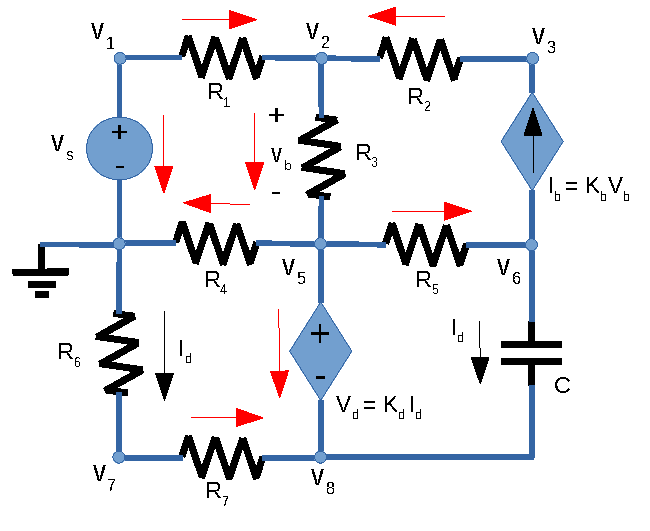
\includegraphics[width=0.4\linewidth]{mcurrents.pdf}
\caption{Circuit with each current direction arbitrarily assigned, to assist in the analysis of the circuit by the Nodal Method.}
\label{fig:nvoltages}
\end{figure}

For t\textless 0, -t\textgreater 0. Because of that u(t)=0 and u(-t)=1. So:
\begin{equation}
  v_S(t<0)=V_s
\end{equation}

That means that the voltage source drives constant voltage $V_s$, in other words, the voltage doesn't varies in time.
Consequently, the current of the capacitor is null:
\begin{equation}
  I_c=0
\end{equation}

To determine the nodal voltages, we use the nodal method.

We first start by calculating the values of the conductances of the various resistors:
\begin{equation}
  G_i=1/R_i
\end{equation}

Then we determine the KCL equations in nodes not connected to voltage sources and another additional equations for nodes 
related by voltage sources.

After doing that we can now obtain the matricial equation wich will allow us to determine de nodal voltages:

\begin{gather}
	\begin{bmatrix}
		1 & -0 & 0 & 0 & 0 & 0 & 0 \\
		G_1 & -G_1 - G_2 - G_3 & G_2 & G_3 & 0 & 0 & 0 \\
		0 & G_2 + K_b & -G_2 & -K_b & 0 & 0 & 0 \\
		0 & -G_3 & 0 & G_3+G_4+G_5 & -G_5 & -G_7 & G_7 \\
		0 & -K_b & 0 & G_5+K_b & -G_5 & 0 & 0 \\
		0 & 0 & 0 & 0 & 0 & -G_6-G_7 & -G_7 \\
		0 & 0 & 0 & 1 & 0 & G_6\cdot K_d & -1 \\
	\end{bmatrix}
	\begin {bmatrix} V_1 \\ V_2 \\ V_3 \\ V_5  \\ V_6 \\ V_7 \\ V_8 \end{bmatrix}
	=
	\begin {bmatrix} V_s  \\ 0  \\ 0  \\ 0 \\ 0  \\ 0 \\ 0 \end{bmatrix}
\end{gather}

The solution of this matricial equation is determined by Octave:
\begin{table}[H]
  \centering
  \begin{tabular}{|l|r|}
    \hline    
    {\bf Node} & {\bf Voltage[V]} \\ \hline
    $V_{1}$ & 1.726209e+00 \\ \hline
$V_{2}$ & -2.924287e-01 \\ \hline
$V_{3}$ & -4.528138e+00 \\ \hline
$V_{4}$ & 9.535580e+00 \\ \hline
$V_{5}$ & 9.279827e-06 \\ \hline
$V_{6}$ & -1.191502e+00 \\ \hline
$V_{7}$ & -3.522212e+00 \\ \hline

  \end{tabular}
  \caption{Nodal Voltages Values}
  \label{tab:nodal}
\end{table}

Knowing these voltages, it is also possible to determine branch currents, using Ohm’s Law and Kirchoff's Laws.
Note that:
\begin{equation}
  I_S=I_1
\end{equation}
\begin{equation}
  I_{Vd}=-I_7
 \end{equation}
 \begin{equation}
  I_b=K_b\cdot(V_2-V_5)
\end{equation}
 
 \begin{table}[H]
  \centering
  \begin{tabular}{|l|r|}
    \hline    
    {\bf Name} & {\bf Current[A]} \\ \hline
    $V_{b}$ & -2.924287e-01 \\ \hline
$I_{b}$ & -2.109620e-03 \\ \hline
$V_{c}$ & -9.279827e-06 \\ \hline
$I_{c}$ & -1.157872e-03 \\ \hline
$I_{R1}$ & -2.015673e-03 \\ \hline
$I_{R2}$ & -2.109620e-03 \\ \hline
$I_{R3}$ & -9.394704e-05 \\ \hline
$I_{R4}$ & 8.578007e-04 \\ \hline
$I_{R5}$ & 3.150480e-03 \\ \hline
$I_{R6}$ & -1.157872e-03 \\ \hline
$I_{R7}$ & -1.157872e-03 \\ \hline

  \end{tabular}
  \caption{Currents of circuit components}
  \label{tab:valn}
\end{table}

\subsection{Equivalent Resistance, $R_{eq}$}
The objective of this task is to calculate $R_{eq}$ as seen in terminals of the capacitor. That can be useful to study the circuit and the variation of its nodal values for t = 0.
In order to solve it, we used the concept of the Thévenin and Norton Theorems.\par
These theorems state that all linear circuits of sources and resistors can be substituted by a simpler circuit with an equivalent resistor and a voltage or current source, respectively, from a chosen point of view.

In that way, we first replaced the capcitor by an independent voltage source $V_x$ and, then, we put the independent voltage source $V_s$ to 0V. It is important to notice that the depedent voltage source cannot be put equal to 0V and the dependent current source cannot be removed from the circuit.

The analysed circuit is represented on figure ~\ref{fig:circuit22}.

\begin{figure}[H] \centering
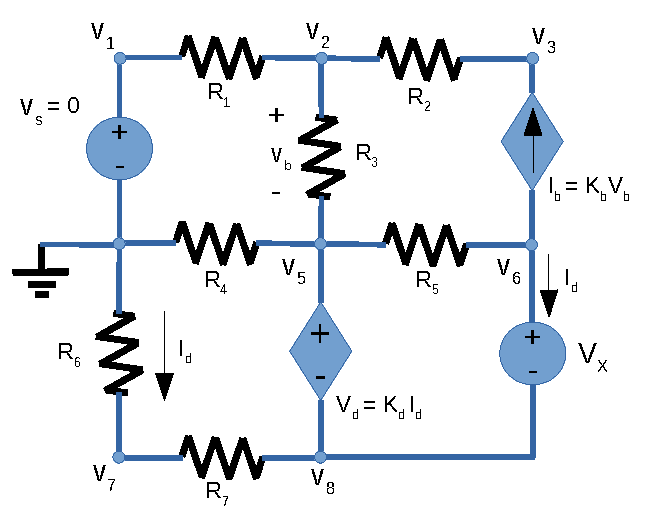
\includegraphics[width=0.4\linewidth]{nvoltages.pdf}
\caption{Circuit Analysed}
\label{fig:circuit22}
\end{figure}

Although the voltage in the nodes is not necessarily continuous, the difference pottencial in the capacitor, wich is given by the difference between nodes 6 and 8, is.
Therefore, we considered:
\begin{equation}
   V_{x}= V_6-V_8
\end{equation}
, where $V_6$ and $V_8$ are the voltages in nodes 6 and 8 obtained in the previous subsection.

Then, we run the node analysis to determine the current $I_x$ in order to determine the $R_{eq}$ by using Ohm's Law:
\begin{equation}
   R_{eq}= \frac{V_x}{I_x}
\end{equation}

This way, we can also determine the time constante:
\begin{equation}
   \tau = R_{eq} \cdot C
\end{equation}

The matrix equation used in the octave tool is the following:
\begin{gather}
	\begin{bmatrix}
		1 & 0 & 0 & 0 & 0 & 0 & 0 \\
		G_1 & -G_1 - G_2 - G_3 & G_2 & G_3 & 0 & 0 & 0 \\
		0 & G_2 + K_b & -G_2 & -K_b & 0 & 0 & 0 \\
		-G_1 & G_1 & 0 & G_4 & 0 & G_6 & 0 \\
		0 & 0 & 0 & 1 & 0 & G_6\cdot K_d & -1 \\
		0 & 0 & 0 & 0 & 1 & 0 & -1 \\
		0 & 0 & 0 & 0 & 0 & -G_6-G_7 & G_7 \\
	\end{bmatrix}
	\begin {bmatrix} V_1 \\ V_2 \\ V_3 \\ V_5  \\ V_6 \\ V_7 \\ V_8 \end{bmatrix}
	=
	\begin {bmatrix} 0  \\ 0  \\ 0  \\ 0 \\ 0  \\ V_x \\ 0 \end{bmatrix}
\end{gather}
And the results obtained are expressed in this table:
\begin{table}[H]
  \centering
  \begin{tabular}{|l|r|}
    \hline    
    {\bf Name} & {\bf Value [A or V]} \\ \hline
    $V_{1}$ & 0.000000e+00 \\ \hline
$V_{2}$ & 0.000000e+00 \\ \hline
$V_{3}$ & 0.000000e+00 \\ \hline
$V_{5}$ & 0.000000e+00 \\ \hline
$V_{6}$ & 8.843309e+00 \\ \hline
$V_{7}$ & -0.000000e+00 \\ \hline
$V_{8}$ & 0.000000e+00 \\ \hline

  \end{tabular}
  \caption{Voltages and currents of circuit components}
  \label{tab:val21}
\end{table}

\begin{table}[H]
  \centering
  \begin{tabular}{|l|r|}
    \hline    
    $V_{x}$ & 8.843309e+00 \\ \hline
$I_{x}$ & 2.921760e-03 \\ \hline
$R_{eq}$ & 3.026707e+03 \\ \hline

  \end{tabular}
  \caption{Calculated Values}
  \label{tab:val22}
\end{table}

\subsection{Natural Solution, $t \geqslant $ 0}

This tasks' objective is to compute the natural solution of the voltage in node 6. Using the results previously obtained in task 2, we  obtained the value of the voltage in this node when t= 0 seconds and $v_{6n}$(t=0s)=$V_x$ , since the result obtain for v8 is zero in the previous task.

\par The natural solution as the following format:
\begin{equation}
v_n(t) = A \cdot \exp(\frac{-t}{RC})
\end{equation}

In this particular case, A= $v_6$(t=0) =$V_x$, giving us the equation below:

\begin{equation}
v_6n(t) = V_x \cdot \exp(\frac{-t}{RC})
\end{equation}

The following plot was obtained using the octave tool and it shows the graph obtained for the natural solution of the voltage in node 6 and it is as expected a negative exponetial:
\begin{figure}[H] \centering
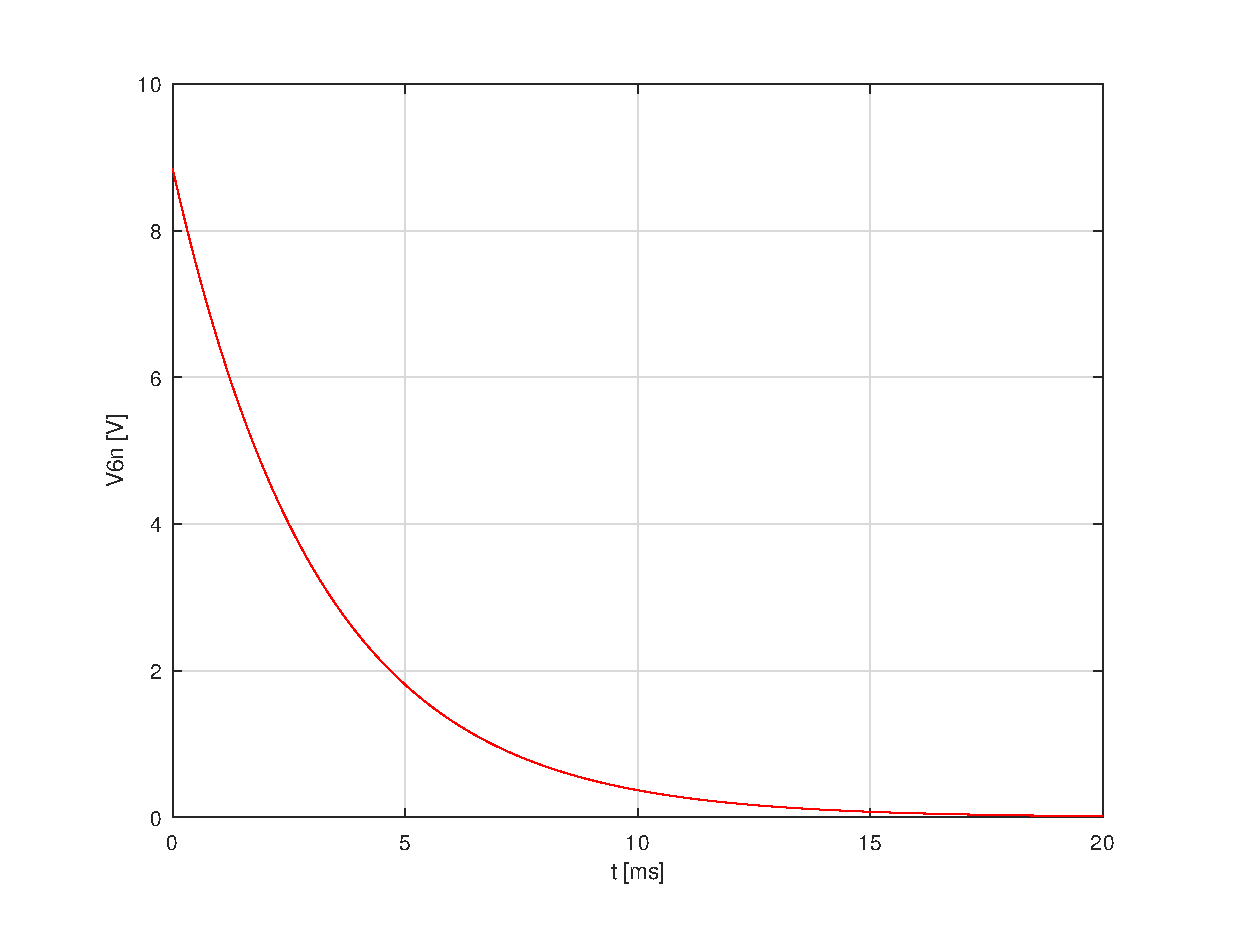
\includegraphics[width=0.6\linewidth]{theoretical.eps}
\caption{Natural response.}
\label{fig:point3}
\end{figure}

\subsection{Point 4}
In order to compute the forced solution for the voltage in node 6,it was utilized the same time interval considered in the previous task.
\par But to calculate the forced solution, we need to used the regular circuit and to do that we assumed a phasor Vs and substituited the capacitor C for its impedance, Zc.
\par The phasor used was:
\begin{equation}
V_s = \exp(-i\cdot \frac{pi}{2})
\end{equation}
And the formula to obtain Zc is:
\begin{equation}
Z_c= \frac{1}{i\cdot C \cdot \omega}
\end{equation}
With all of that taken into consideration, the matrix equation used to calculate the forced solution in this time interval is the following:
\begin{gather}
	\begin{bmatrix}
		1 & 0 & 0 & 0 & 0 & 0 & 0 \\
		-G_1 & G_1 & 0 & G_4 & 0 & G_6 & 0 \\
		G_1 & -G_1 & -G_2 & -K_b & 0 & 0 & 0 \\
		0 & G_2+Kb & -G_2 & -K_b & 0 & 0 & 0;\\
               0 & -Kb & 0 & Kb+G_5 & -G_5-\frac{1}{Z_c} & 0 & \frac{1}{Z_c} \\
               0 & 0 & 0 & 0 & 0 & -G_6-G_7 & G_7\\
               0 & 0 & 0 & 1 & 0 & G_6\cdot K_d &-1\\
	\end{bmatrix}
	\begin {bmatrix} V_1 \\ V_2 \\ V_3 \\ V_5  \\ V_6 \\ V_7 \\ V_8 \end{bmatrix}
	=
	\begin {bmatrix} 0  \\ 0  \\ 0  \\ 0 \\ 0  \\ V_x \\ 0 \end{bmatrix}
\end{gather}
The result obtained can be seen in the plot below:

\begin{figure}[H] \centering
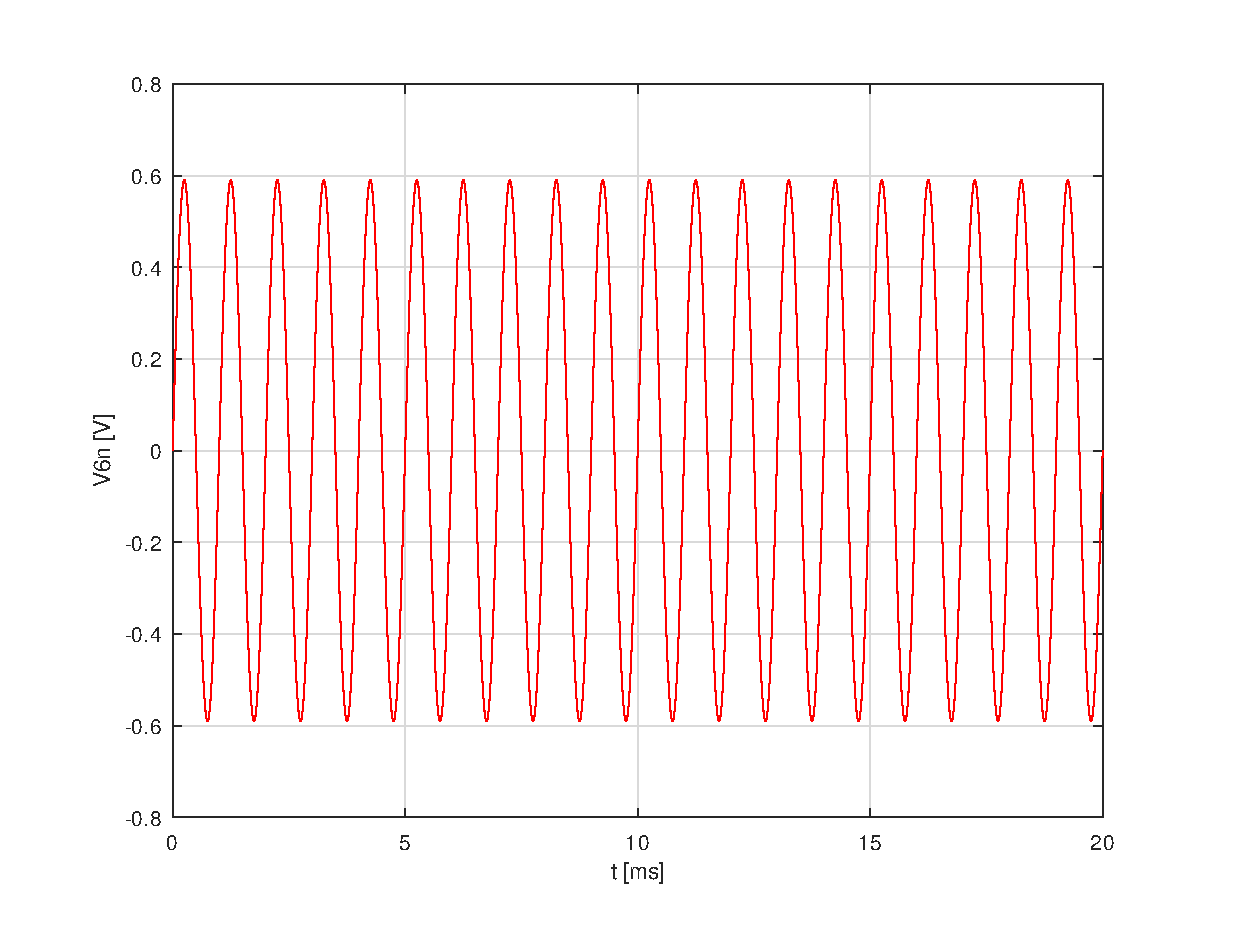
\includegraphics[width=0.6\linewidth]{Forced4.eps}
\caption{Final response.}
\label{fig:point4}
\end{figure}

The phasor amplitude values and phases were also computed in this task and can be consulted in the Table (X):
\begin{table}[H]
  \centering
  \begin{tabular}{|l|r|}
    \hline    
    {\bf Name} & {\bf Value [A or V]} \\ \hline
    $V_{1}$ & 1.000000e+00 \\ \hline
$V_{2}$ & 9.589907e-01 \\ \hline
$V_{3}$ & 8.729409e-01 \\ \hline
$V_{5}$ & 9.649315e-01 \\ \hline
$V_{6}$ & 5.902978e-01 \\ \hline
$V_{7}$ & 3.906094e-01 \\ \hline
$V_{8}$ & 5.902978e-01 \\ \hline

  \end{tabular}
  \caption{Amp}
  \label{tab:amp}
\end{table}

\begin{table}[H]
  \centering
  \begin{tabular}{|l|r|}
    \hline    
    {\bf Name} & {\bf Value [A or V]} \\ \hline
    $V_{1}$ & -1.570796e+00 \\ \hline
$V_{2}$ & -1.570796e+00 \\ \hline
$V_{3}$ & -1.570796e+00 \\ \hline
$V_{5}$ & -1.570796e+00 \\ \hline
$V_{6}$ & 1.570802e+00 \\ \hline
$V_{7}$ & 1.570796e+00 \\ \hline
$V_{8}$ & 1.570796e+00 \\ \hline

  \end{tabular}
  \caption{Voltages and currents of some circuit components}
  \label{tab:phases}
\end{table}

\subsection{Point 5}
The total solution for the node 6 for a frequency,f = 1000 Hz was calculated by superimposing
the forced and the natural solution for t maior ou igual 0. For t menor0 , the voltage in node 6 is the
one calculated in the first task. This gives us the following function for v6:

%\begin{equation}
%v_6t
%\begin {cases}
%V_6 & $t$ <0 \\
%v_6n + v_6A * cos(\omega *t - v_6Ph)
%\end{cases}
%\end{equation}

The total solution was plotted together with vs and this is the result obtained:

\begin{figure}[H] \centering
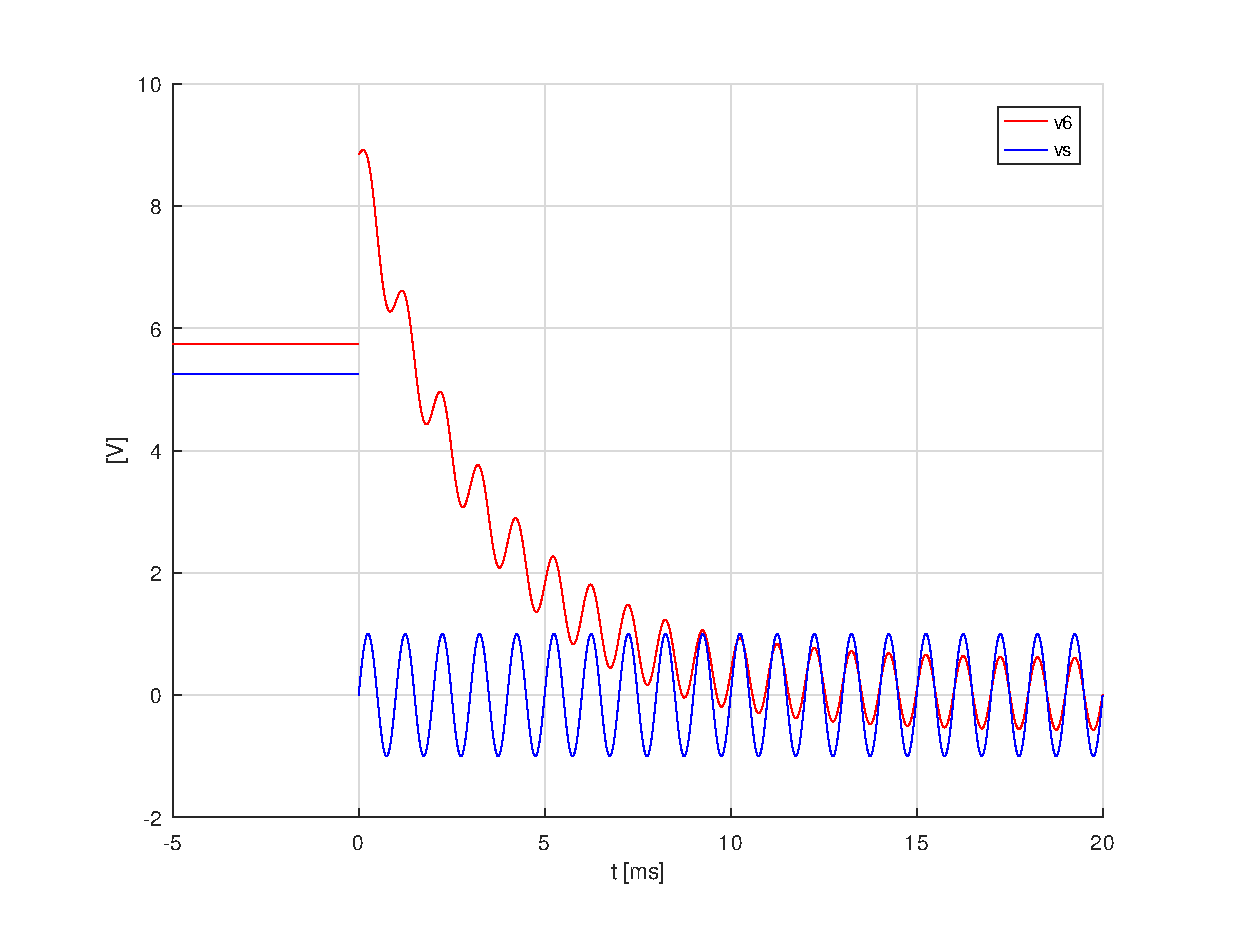
\includegraphics[width=0.6\linewidth]{Theoretical5.eps}
\caption{Final response.}
\label{fig:point5}
\end{figure}

It is worth noticing that v6t is not continuous.

\subsection{Point 6}
The last assignment is to study how the amplitude ,in decibels, and the phase, in degrees, of v6, vs and vc= v6 - v8 vary with different frequencies. In order to achieve this objective, we plotted this fuctions together twice, in one of them we study the variance of the amplitude (Figure X) and in the other the variance of the phase (Figure Y). To obtain the intervals we used the logspace in the range of 0,1 Hz to 1 MHz.
\par Plot studying the amplitude variance:
\begin{figure}[H] \centering
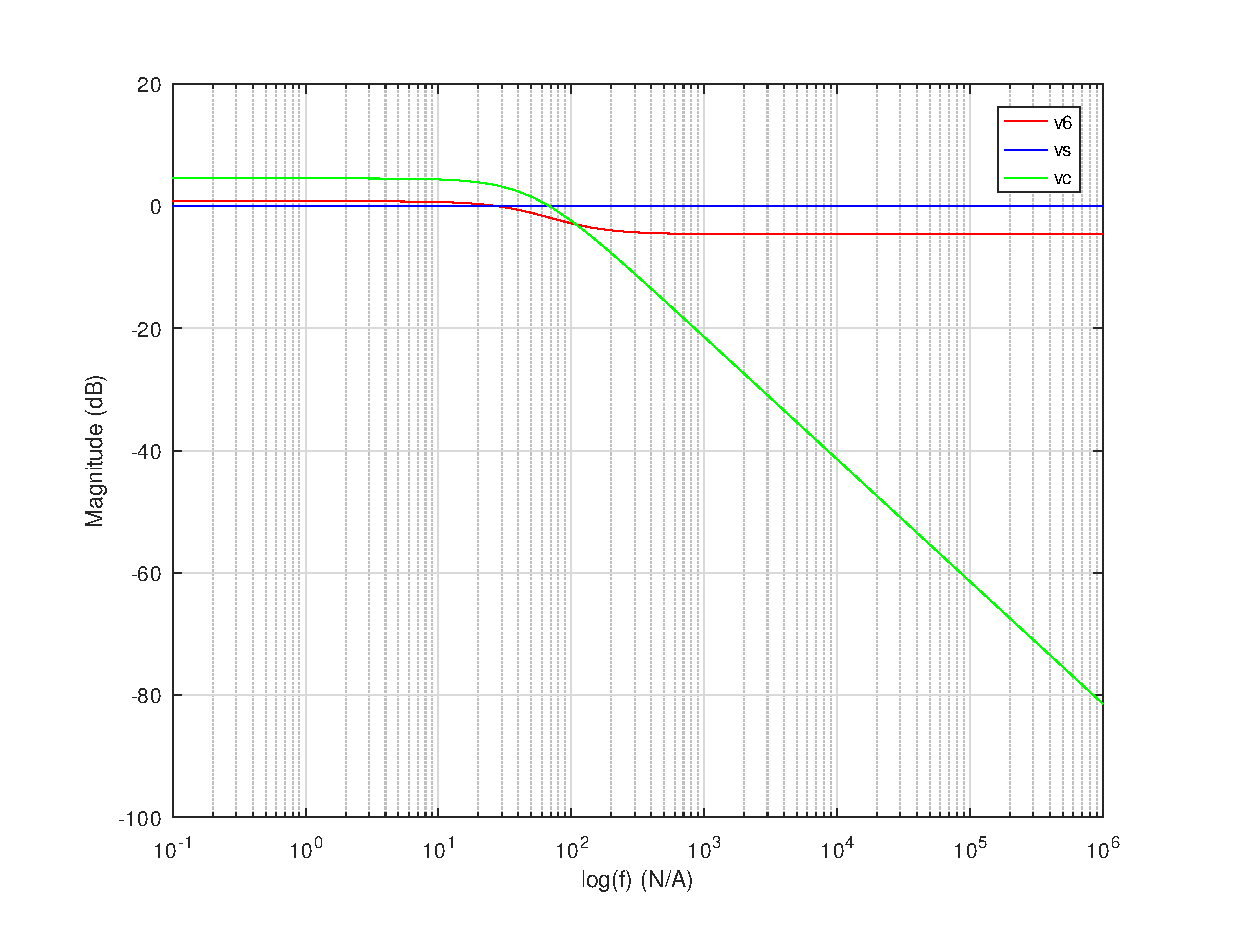
\includegraphics[width=0.6\linewidth]{freq6SC.eps}
\caption{Final response.}
\label{fig:point61}
\end{figure}
Since the transfer function is calculated via a quocient of the output and the input, the result expected and obtained for vs is zero.
It is also noticeable that vc rapidly decreases as the frenquency shoots upwards.\par
Regarding v6, it is noticeable that for higher frequencies that the functions is constant, this is due to the fact that for this kind of frequencies the capacitator
acts as a shunt, meaning that only the resistors (that do not vary with the frequency) influence the variance, making it constant. For lower frequencies, it is observable that
there is a slightly decrease. This is expected in a RC circuit and it is due to the impedance of the capacitor.

Plot studying the phase variance:\par
\begin{figure}[H] \centering
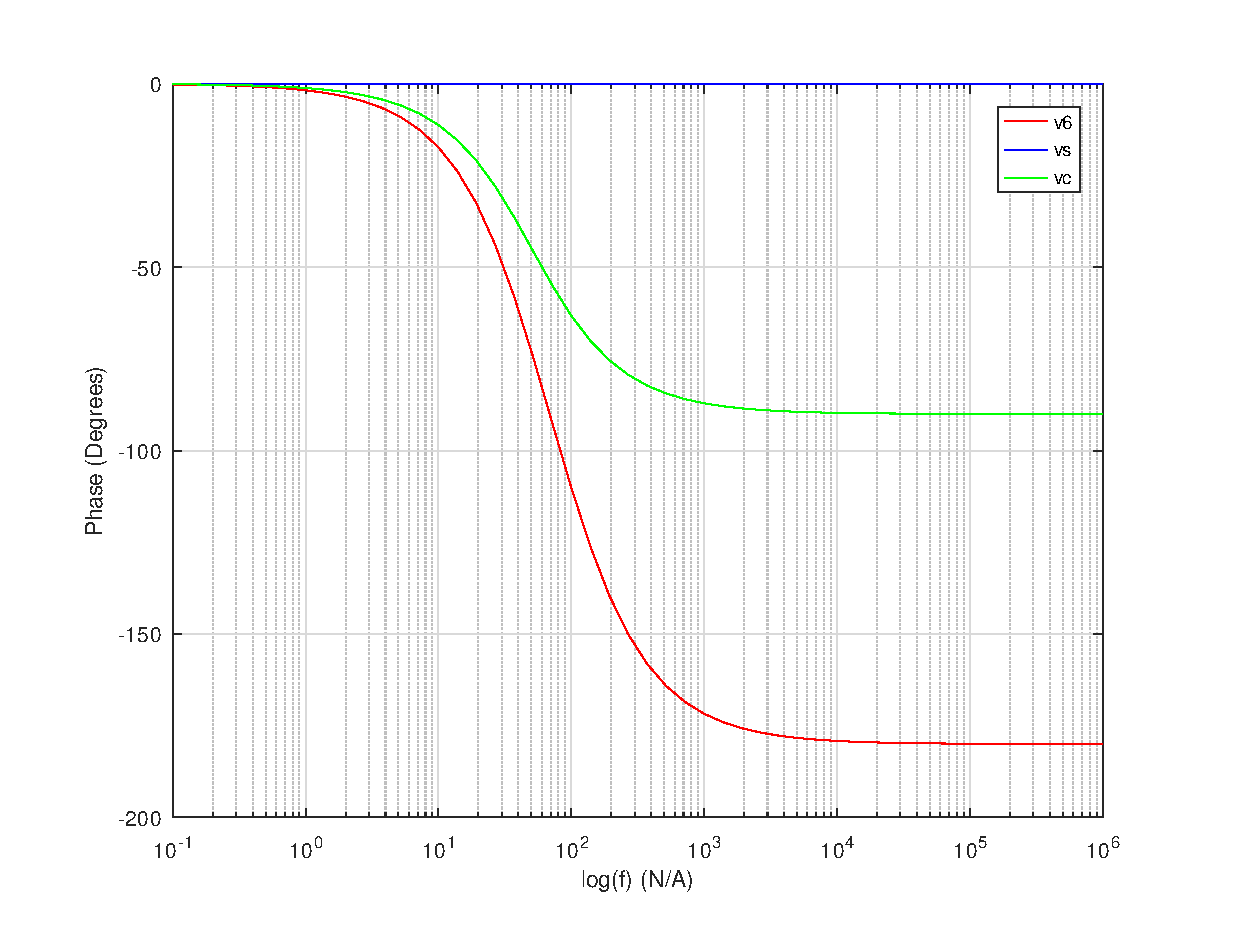
\includegraphics[width=0.6\linewidth]{ph6SC.eps}
\caption{Final response.}
\label{fig:point62}
\end{figure}
It is worth noticing that, as expected , the phase variance of vs is null. This is also due to the fact that the transfer function is calculated using a quocient between the output and the input.
For v6 and vc, it is observable that with the frequency increment the phase achieve lower values and are all negative, as expected. 
